\documentclass[12pt,letterpaper]{article}

\usepackage{graphicx,fontspec,anyfontsize,array,tabularx}
\usepackage[T1]{fontenc}
\usepackage[all]{nowidow}

\usepackage[margin=1in, headheight=18pt, headsep=12pt]{geometry}

\usepackage{xcolor}
\definecolor{black}{RGB}{0, 0, 0}
\definecolor{blue_links}{RGB}{0, 0, 238}

\usepackage[
    colorlinks=true,
    allcolors=blue_links,
    bookmarks=false,
    pdfstartview={XYZ null null 1.00}
]{hyperref}

\usepackage[
    backend=biber,
    sorting=nyt
]{biblatex}
\addbibresource{cite_diffusion_tricks.bib}

\setmainfont{Times New Roman}
\setmonofont{Cascadia Code}

\usepackage{fancyhdr,lastpage}
\pagestyle{fancy}
\fancyhf{}
\fancyfoot[C]{\thepage{} of \pageref*{LastPage}}

\begin{document}
    \renewcommand{\headrulewidth}{0pt}
    \color{black}
    \setlength{\parskip}{12pt}

    \noindent
    \underline{\fontsize{16}{19.2}\selectfont{}Advanced Artificial Intelligence -- Diffusion Tricks Project}\\[4pt]
    Joey Sodergren and Akash Prasad -- May 5\textsuperscript{th}, 2025

    Our project implements a modified diffusion system which is capable of generating dual perception images that satisfy two different textual prompts simultaneously. Our approach is built on SDXL-Turbo \cite{sdxl_turbo}, which is an improved and distilled version of Stable Diffusion, as inspired by "Diffusion Illusions" by Burgert et al \cite{diffusion_illusions}. The model generates an image that appears to satisfy one prompt when viewed normally, and another prompt when it is transformed through rotation, mirroring or splitting the image into pieces and rearranging them.

    The motivation for this research and experimentation stems mostly from technical curiosity, but it may have some practical applications. From a technical perspective, this project explores the boundaries of what diffusion models can achieve beyond conventional single-prompt image generation. The challenge of synchronizing two different visual representations within one coherent image pushes these models into new territory. From a practical standpoint, dual-perception images offer intriguing applications in creative arts, visual communication, and potentially even information hiding.

    \noindent\textbf{Inputs and Outputs}\setlength{\parskip}{0pt}

    Our system requires four primary inputs: two distinct text prompts (Prompt A and Prompt B), a bitmap transformation method (such as rotation, mirroring, or pixel rearrangement), and a bitmap un-transformation method (which should perfectly undo the effect of the first transformation method). The output is a single image that, when viewed normally, appears to satisfy Prompt A, and when transformed according to the specified method, satisfies Prompt B. The core of our implementation leverages SDXL-Turbo \cite{sdxl_turbo}, which we run on consumer-grade NVIDIA hardware with 8GB VRAM, making this research accessible without requiring highly-specialized computing infrastructure.\setlength{\parskip}{12pt}

    \noindent\textbf{Diffusion Model Selection}\setlength{\parskip}{0pt}

    From the outset, we agreed that utilizing a competent pre-trained model would be the most efficient approach to this project. It was for that reason that we initially explored using the SDXL model as our generative backend. According to Podell et al. \cite{sdxl}, SDXL was trained on a diverse collection of high-quality images with associated text descriptions, and even though the complete details of its training data are not fully disclosed, we were confident SDXL could produce outputs of sufficient quality to support our use-case.\setlength{\parskip}{12pt}

    However, after initial experiments had concluded, we noted a few concerns regarding the usage of SDXL. Out of the box, its default iteration number of 50 produced extremely pleasing images, but required more time and more VRAM than we liked. In order to accelerate our iteration time to allow more efficient experimentation and trial-and-error adjustments of our process, we switched to SDXL-Turbo, which is a ``distilled'' version of SDXL that enables ``sampling large-scale foundational image diffusion models in 1 to 4 steps at high image quality'' \cite{sdxl_turbo}. This allowed us to drastically shrink the number of inference steps used at each stage in our image generation process.

    \newpage
    \noindent\textbf{High-Level Process Description}\setlength{\parskip}{0pt}

    We will now describe from a high-level perspective the image generation process that our project implements. First, we need to define our major terms and variables:
    \begin{itemize}
        \setlength{\itemsep}{0pt}
        \item \texttt{prompt\_a} is a string, containing the image generation prompt used for the untransformed view of the image.
        \item \texttt{prompt\_b} is a string, containing the image generation prompt used for the transformed view of the image.
        \item \texttt{transform\_img} is a function that takes in a bitmap image and transforms the locations of its pixels.
        \item \texttt{untransform\_img} is a function that takes in a bitmap image and transforms the locations of its pixels, in such a manner that it perfectly undoes the transform performed by \texttt{transform\_img}.
        \item \texttt{strength\_schedule} is a list of numbers, defined as follows:\\\lbrack0.98, 0.9, 0.8, 0.7, 0.6, 0.5, 0.4, 0.3, 0.2, 0.1\rbrack
        \item \texttt{steps\_schedule} is a list of numbers, defined as follows:\\\lbrack4, 4, 4, 5, 5, 6, 7, 8, 9, 10\rbrack
        \item \texttt{img\_a} is a bitmap image, which always contains the most recent untransformed image result.
        \item \texttt{img\_b} is a bitmap image, which always contains the most recent transformed image result.
    \end{itemize}

    \noindent{}The image generation process then proceeds in this manner:
    \begin{enumerate}
        \setlength{\itemsep}{0pt}
        \item \texttt{img\_a} is initialized to random noise, as generated by \\\texttt{numpy.random.random\_sample()}.
        \item \texttt{img\_b} is initialized to \texttt{transform\_img(img\_a)}.
        \item For \texttt{i} in \texttt{range(10)}, repeat the following steps:
        \begin{enumerate}
            \item The contents of \texttt{img\_a} are replaced with the result of an execution of SDXL-Turbo's image-to-image mode, with the following key parameters:
            \begin{itemize}
                \item Inference shall use the current contents of \texttt{img\_a} as its base state.
                \item Inference shall use \texttt{prompt\_a} as its textual target.
                \item Before inference, SDXL-Turbo will add noise to the base image of the amount specified by \texttt{strength\_schedule[i]}.
                \item \texttt{num\_inference\_steps} is specified to be \texttt{steps\_schedule[i]}. (This was as recommended by the SDXL-Turbo description \cite{sdxl_turbo}, which states that we should ensure that the number of steps multiplied by the noise strength should always be greater than or equal to 1.)
            \end{itemize}
            \item The contents of \texttt{img\_b} are replaced with the result of another execution of SDXL-Turbo's image-to-image mode, with the following key parameters:
            \begin{itemize}
                \item Inference shall use the current contents of \texttt{img\_b} as its base state.
                \item Inference shall use \texttt{prompt\_b} as its textual target.
                \item Before inference, SDXL-Turbo will add noise to the base image of the amount specified by \texttt{strength\_schedule[i]}.
                \item \texttt{num\_inference\_steps} is specified to be \texttt{steps\_schedule[i]}.
            \end{itemize}
            \item \texttt{img\_b} is now replaced with \texttt{untransform\_img(img\_b)}.
            \item \texttt{img\_a} and \texttt{img\_b} are now merged together to produce \texttt{img\_smash}.
            \begin{itemize}
                \item The precise method for recombining the images is a custom process that we produced, which takes the average of the two images, and then readjusts the per-channel values of the result to maximize contrast. More on this process will be discussed further below.
            \end{itemize}
            \item \texttt{img\_a} is now replaced with \texttt{img\_smash}.
            \item \texttt{img\_b} is now replaced with \texttt{transform\_img(img\_smash)}.
            \item \texttt{img\_a} and \texttt{img\_b} are now written out to PNG files for human monitoring and review.
        \end{enumerate}
    \end{enumerate}

    \noindent\textbf{Example Image Results}\setlength{\parskip}{0pt}

    The following are a few cherry-picked image results produced by our software that we considered to be satisfactory. Relevant generation parameters are provided below each image.\setlength{\parskip}{12pt}

    \noindent\begin{tabular}{ >{\centering}m{2.9in} m{0.18in} >{\centering\arraybackslash}m{2.9in} }
        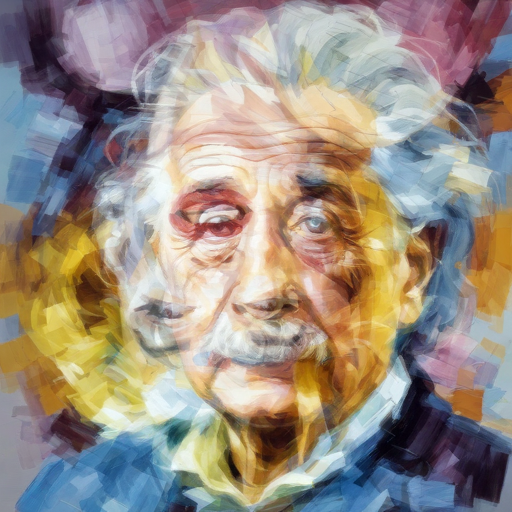
\includegraphics[width=2.8in]{img_einstein_monroe_7.png} & & 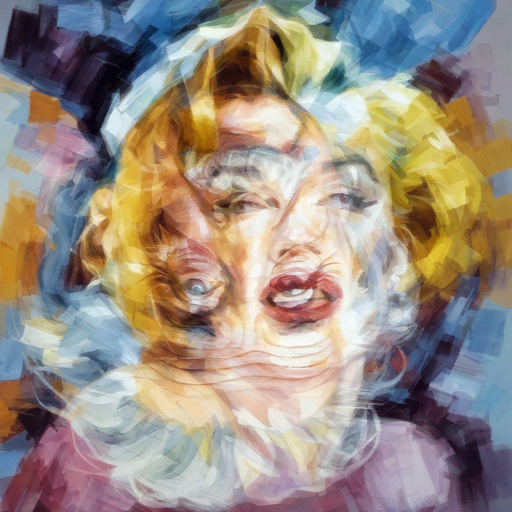
\includegraphics[width=2.8in]{img_einstein_monroe_7_rotated.png} \\
        Right side up prompt: ``Albert Einstein, impressionist painting, 8k'' & & Same image, rotated upside down. \\
        Upside down prompt: ``Marilyn Monroe, impressionist painting, 8k'' & & \\
        Selected result at stage 7. & & \\
    \end{tabular}

    Of particular note in this result are the features of the image that serve double purposes. The yellow of Monroe's blonde hair was integrated into Einstein as a warm light being cast on one side of his face, and on his neck. The dark shading under Einstein's chin was integrated into the shading of curls in Monroe's hair. Monroe's chin also seems to have correlated itself with the wrinkles in Einstein's forehead.

    \noindent\begin{tabular}{ >{\centering}m{2.9in} m{0.18in} >{\centering\arraybackslash}m{2.9in} }
        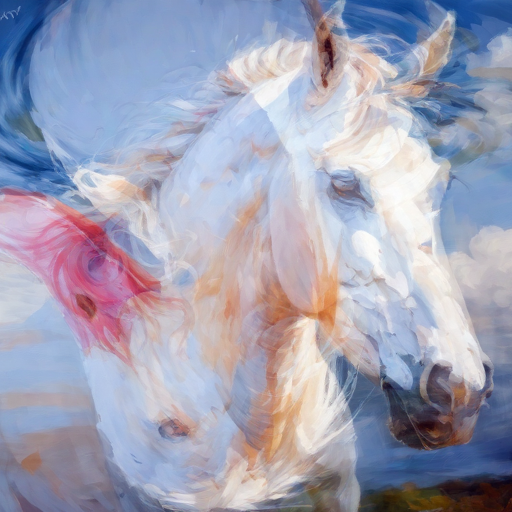
\includegraphics[width=2.8in]{img_horse_duck_6.png} & & 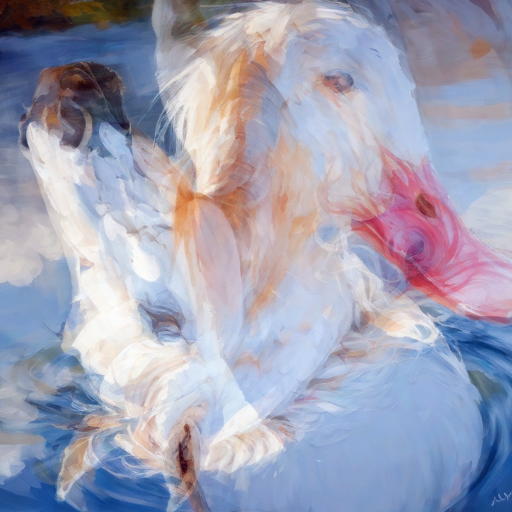
\includegraphics[width=2.8in]{img_horse_duck_6_rotated.png} \\
        Right side up prompt: ``white horse, close up, face, impressionist painting, 8k'' & & Same image, rotated upside down. \\
        Upside down prompt: ``white duck, close up, face, head, feathers, impressionist painting, 8k'' & & \\
        Selected result at stage 6. & & \\
    \end{tabular}

    The above result is an example of an image merge that's slightly more noticeable than we desired. The duck's brightly colored bill and the horse's dark muzzle are particularly difficult to contextually hide, and stand out in both rotations of the image.

    \noindent\begin{tabular}{ >{\centering}m{2.9in} m{0.18in} >{\centering\arraybackslash}m{2.9in} }
        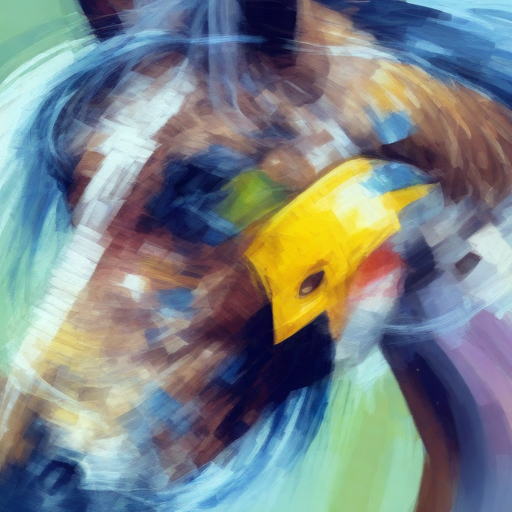
\includegraphics[width=2.8in]{img_brown_horse_duck_8.png} & & 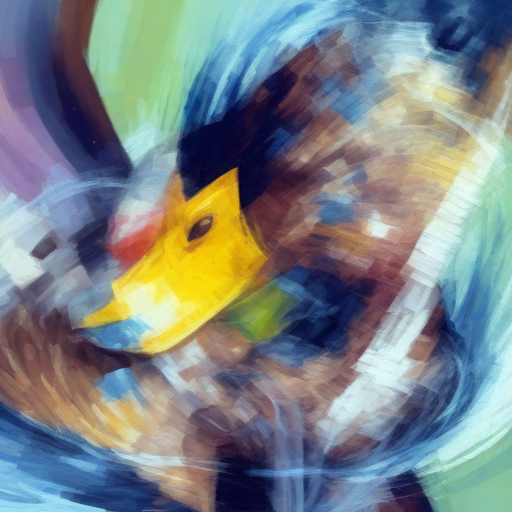
\includegraphics[width=2.8in]{img_brown_horse_duck_8_rotated.png} \\
        Right side up prompt: ``horse, close up, face, impressionist painting, 8k'' & & Same image, rotated upside down. \\
        Upside down prompt: ``duck, close up, face, head, impressionist painting, 8k'' & & \\
        Selected result at stage 8. & & \\
    \end{tabular}

    Removing a few terms from the prompts produced the above result, which we found to be more visually pleasing. The horse's snout and the duck's head correlated well, as did the duck's feathers with the horse's mane. We did experiment with adding ``facing left'' and ``facing right'' to image prompts in order to attempt a directed alignment of image features, but SDXL-Turbo consistently disregarded such instructions.

    \noindent\textbf{Trial and Error}\setlength{\parskip}{0pt}

    To wrap up, we'd like to describe a few facets of our development process and our findings when inspecting results in detail. We'll begin by providing here one particularly bad result we got following the completion of our very first version of the two-prompt generation process:

    \noindent\begin{center}
        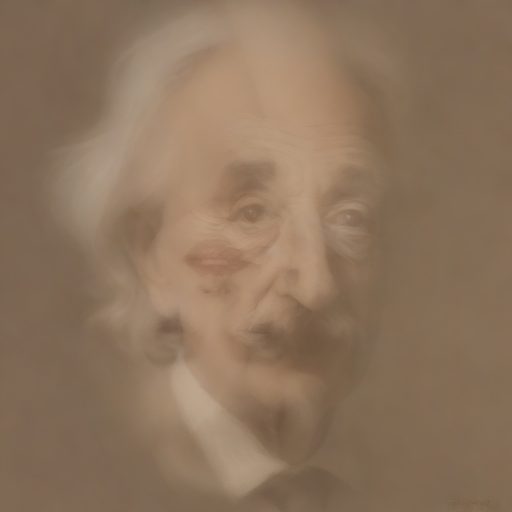
\includegraphics[width=2.8in]{img_einstein_monroe_muddy.png}
    \end{center}

    At the time that this image was generated, the process we were using to recombine \texttt{img\_a} and \texttt{img\_b} was simply to take the literal average of corresponding color channels in each pixel of the two images. We quickly realized that this was an insufficient process, as any average of two numbers in between 0 and 1 will trend towards 0.5 (or in other words, towards grey), and this trend would compound itself over the multiple steps in our generation schedule.\setlength{\parskip}{12pt}

    In order to remedy this flaw, we developed a new image recombination method that \emph{begins} with taking the average of corresponding pixels, and then finds the minimum and maximum values in each of the red, green, and blue channels across the whole image. The values of each channel in each pixel are then rescaled so that the darkest and brightest values in each channel are stretched out to 0 and 1. (The specifics of this process can be found in the \texttt{recombine\_images()} function in our source code.)

    Immediately after making those upgrades to the image recombination process, the next generation attempt we ran yielded the result shown on page 3. We'd now like to call attention to why we cherry-picked the result from stage 7 of that generation. Our testing indicates that running SDXL-Turbo on the same (or similar) input image too many times can begin to harm the quality of the result. Case in point, here's a comparison of the stage 7 result from page 3 (our favorite of this particular generation), and the stage 9 result from the same generation (the result of the last iteration).

    \noindent\begin{tabular}{ >{\centering}m{2.9in} m{0.18in} >{\centering\arraybackslash}m{2.9in} }
        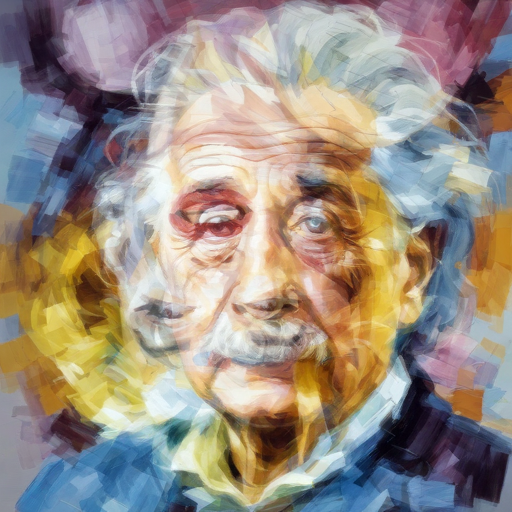
\includegraphics[width=2.8in]{img_einstein_monroe_7.png} & & 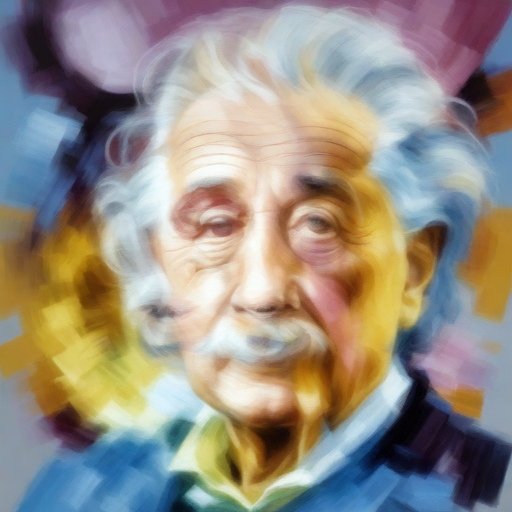
\includegraphics[width=2.8in]{img_einstein_monroe_9.png} \\
        Selected result at stage 7. & & Selected result at stage 9. \\
        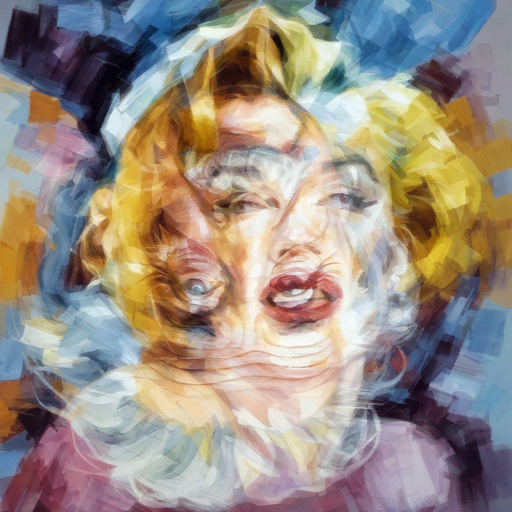
\includegraphics[width=2.8in]{img_einstein_monroe_7_rotated.png} & & 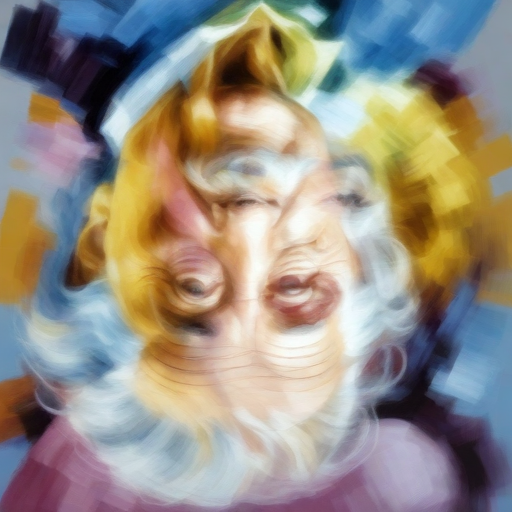
\includegraphics[width=2.8in]{img_einstein_monroe_9_rotated.png} \\
        Upside down result at stage 7. & & Upside down result at stage 9. \\
    \end{tabular}

    We consider the stage 9 output to be inferior to the stage 7 output, as it looks smoother than the prompted ``impressionist painting'' style would reasonably warrant, and has compromised some of the recognizability of Monroe's face while prioritizing Einstein's face. We performed other tests in which we asked for other styles, and we also experimented with adding a jump back \emph{up} in noise intensity into the schedule. These tests were unsuccessful at remedying the issue: after a certain number of iterations of our process, one of the prompts will often start being prioritized over the other prompt.

    This flaw highlights one of the big differences between the original Diffusion Illusions \cite{diffusion_illusions} process and our own, much more simplified version. The Diffusion Illusions process involves the usage of multiple attempts of inference at the same timestep, the results of which are then graded for their similarity to prime ``dream targets''. Our process does not include this regression process, which makes our project faster but also more volatile, and less guaranteed to produce consistently pleasing results.

    \setlength{\parskip}{0pt}
    \printbibliography

\end{document}
